\section{Deriving a pure functional approach}
\label{sec:functional_approach}

%2 main points from Henrik: 1.: try to stick to synchronous updates because this is how the real world works. 2.: get rid of globally shared mutable state as it complicates things extremely with reasoning
%clear conceptual formal model of what agents are and then structure my implementation around it

% TODO: put explanations before the code, otherwise readers get confused e.g. stepSimulation function

We presented a high-level agent-based approach to the SIR model in the previous section, which focused only on the states and the transitions, but we haven't talked about technical implementation details on how to actually implement such a state-machine. The authors of \cite{thaler_art_2017} discuss two fundamental problems of implementing an agent-based simulation from a programming language agnostic point of view. The first problem is how agents can be pro-active and the second how interactions and communication between agents can happen. For agents to be pro-active they must be able to perceive the passing of time, which means there must be a concept of an agent-process which executes over time. Interactions between agents can be reduced to the problem of how an agent can expose information about its internal state which can be perceived by other agents. \\
In this section we will derive a pure functional approach for an agent-based simulation of the SIR model in which we will pose solutions to the previously mentiond problems. We will start out with a very naive approach and show its limitations which we overcome by adding FRP. Then in further steps we will add more concepts and generalisations, ending up at the final approach which utilises monadic stream functions (MSF), a generalisation of FRP 
\footnote{The code of all steps can be accessed freely through the following URL: \url{https://github.com/thalerjonathan/phd/tree/master/public/purefunctionalepidemics/code}}.

% TODO: put all functions in italics

\subsection{Step I: Naive beginnings}
In our first step we start with modelling the states of the agents for which we simply use an Algebraic Data Type (ADT):

\begin{minted}[fontsize=\footnotesize]{haskell}
data SIRState = Susceptible | Infected | Recovered
\end{minted}

Also agents are ill for some duration meaning we need to keep track when a potentially infected agent recovers. Also as previously mentioned, a simulation is stepped in discrete or continuous time-steps thus we introduce a notion of \textit{time} and $\Delta t$ by defining:

\begin{minted}[fontsize=\footnotesize]{haskell}
type Time      = Double
type TimeDelta = Double
\end{minted}

Now we can represent every agent simply as a tuple of its SIR-state and its potential recovery time. We hold all our agents simply in a list and define helper functions:
\begin{minted}[fontsize=\footnotesize]{haskell}
type SIRAgent = (SIRState, Time)
type Agents   = [SIRAgent]

is :: SIRState -> SIRAgent -> Bool
is s (s',_) = s == s'

susceptible :: SIRAgent
susceptible = (Susceptible, 0)

infected :: Time -> SIRAgent
infected t = (Infected, t)

recovered :: SIRAgent
recovered = (Recovered, 0)
\end{minted}

Next we need to think about how to actually step our simulation. For this we define a function which simply steps our simulation with a fixed $\Delta t$ until a given time $t$ where in each step the agents are processed and the output is fed back into the next step.
TODO: need a much better explanation and maybe split up into more steps?
As already mentioned in previous sections, the agent-based implementation of the SIR model is inherently stochastic which means we need access to a random-number generator. We decided to use the Rand Monad at this point as threading a generator through the simulation and the agents is very cumbersome. Thus our simulation stepping runs in the Rand Monad:

\begin{minted}[fontsize=\footnotesize]{haskell}
runSimulation :: RandomGen g 
              => Time 
              -> TimeDelta 
              -> Agents 
              -> Rand g [Agents]
runSimulation tEnd dt as = runSimulationAux 0 dt as []
  where
    runSimulationAux :: RandomGen g 
                     => Time 
                     -> TimeDelta 
                     -> Agents 
                     -> [Agents] 
                     -> Rand g [Agents]
    runSimulationAux t dt as acc
      | t >= tEnd = return $ reverse (as : acc)
      | otherwise = do
        as' <- stepSimulation dt as 
        runSimulationAux (t + dt) dt as' (as : acc)

stepSimulation :: RandomGen g => TimeDelta -> Agents -> Rand g Agents
stepSimulation dt as = mapM (processAgent dt as) as
\end{minted}

Now we can implement the behaviour of an individual agent. First we need to distinguish between the agents SIR-states:

\begin{minted}[fontsize=\footnotesize]{haskell}
processAgent :: RandomGen g 
             => TimeDelta 
             -> Agents 
             -> SIRAgent 
             -> Rand g SIRAgent
processAgent _  as    (Susceptible, _) = susceptibleAgent as
processAgent dt _   a@(Infected   , _) = return $ infectedAgent dt a
processAgent _  _   a@(Recovered  , _) = return a
\end{minted}

An agent gets fed all the agents states so it can draw random contacts. Note that this includes also the agent itself thus we would need to omit the agent itself to prevent making contact with itself. We decided against that as it complicates the solution and for larger numbers of agent population the probability for an agent to make contact with itself is so small that it can be neglected.

From our implementation it becomes apparent that only the behaviour of a susceptible agent involves randomness and that a recovered agent is simply a sink: it does nothing - its state stays constant.

Lets look how we can implement the behaviour of a susceptible agent. It simply makes contact on average with a number of other agents and gets infected with a given probability if an agent it has contact with is infected.
When the agent gets infected it calculates also its time of recovery by drawing a random number from the exponential distribution meaning it is ill on average for illnessDuration.

\begin{minted}[fontsize=\footnotesize]{haskell}
susceptibleAgent :: RandomGen g => Agents -> Rand g SIRAgent
susceptibleAgent as = do
    rc <- randomExpM (1 / contactRate)
    cs <- doTimes (floor rc) (makeContact as)
    if elem True cs
      then infect
      else return susceptible

  where
    makeContact :: RandomGen g => Agents -> Rand g Bool
    makeContact as = do
      randContact <- randomElem as
      if (is Infected randContact)
        then randomBoolM infectivity
        else return False

    infect :: RandomGen g => Rand g SIRAgent
    infect = do
      randIllDur  <- randomExpM (1 / illnessDuration)
      return  infected randIllDur
\end{minted}

The infected agent is trivial. It simply recovers after the given illness duration which is implemented as follows:

\begin{minted}[fontsize=\footnotesize]{haskell}
infectedAgent :: TimeDelta -> SIRAgent -> SIRAgent
infectedAgent dt (_, t) 
    | t' <= 0   = recovered
    | otherwise = infected t'
  where
    t' = t - dt  
\end{minted}

\subsubsection{Results}
We run the simulation for $t = 150$ time-units with a fixed $\Delta t = 1.0$. With increasing number of agents the dynamics approach the one of the SD simulation. TODO: add pictures

Reflecting on our first naive approach we can conclude that it already introduced the most fundamental concepts of ABS
\begin{itemize}
	\item Time - the simulation occurs over virtual time which is modelled explicitly divided into \textit{fixed} $\Delta t$ where at each the agents are executed.
	\item Agents - we implement each agent as an individual behaviour which depends on the agents state.
	\item Feedback - the output state of the agent in the current time-step $t$ is the input state for the next time-step $t+1$.
	\item Environment - as environment we implicitly assume a fully-connected network where every agent 'knows' every other agents, including itself and thus can make contact with every other agent (including itself).
	\item Stochasticity - its an inherently stochastic simulation, which is indicated by the Rand Monadic type.
	\item Deterministic - repeated runs with the same initial random-number generator result in same dynamics. This may not come as a surprise but in Haskell we can guarantee that property statically already at compile time because our simulation runs in the Rand monad and NOT in the IO Monad. This guarantees that no external, uncontrollable sources of randomness can interfere with the simulation.
	\item Dynamics - it works as expected: with increasing number of agents our solution approaches the SD dynamics 
\end{itemize}

Nonentheless our approach has also weaknesses and dangers:
\begin{enumerate}
	\item $\Delta t$ is passed explicitly as argument to the agent and needs to be dealt with explicitly. It seems to be not very elegant and a potential source of errors - can we do better and find a more elegant solution? 
	\item The way our agents are represented is not very elegant: the state of the agent is explicitly encoded in an ADT and when processing the agent the function needs always first distinguish between the states. Can we express it in a more implicit, functional way?
	\item The states of all agents of the current step are fed back into every agent in the next step so that an agent can pick its contacts. Although agents cannot change the states, this reveals too much information e.g. the illness duration is of no interest to the other agents. Although we could just feed in the SIRStates without the illness duration, the problem is more of conceptual nature: it should be the agent which decides to whom it reveals which information.
\end{enumerate}

We move now to the next step in which we will address points 1 and 2, point 3 will be solved in step 3.

\subsection{Adding Functional Reactive Programming}
\label{sec:step2_frp}
As shown in the first step, the need to handle $\Delta t$ explicitly can be quite messy, is inelegant and a potential source of errors, also the explicit handling of the state of an agent and its behavioural function is not very functional. We can solve both these weaknesses by switching to the functional reactive programming (FRP) paradigm, because it allows to express systems with discrete and continuous time-semantics. In this step we are focusing on arrowized FRP using the library Yampa. In it, time is handled implicit and cannot be messed with and the whole system is built on the concept of signal-functions (SF). A signal-function is basically a continuation which allows then to capture state using closures. Both these fundamental features allow us to tackle the weaknesses of our first step and push our approach further towards a truly functional approach.

\subsubsection{Short introduction to Yampa}
TODO: introduce FRP / Yampa here

\subsubsection{Implementation}
We start by defining our agents now as a signal-function which receives the states of all agents as input and outputs the state of the agent:

\begin{minted}[fontsize=\footnotesize]{haskell}
type SIRAgent = SF [SIRState] SIRState 
\end{minted}

Now we can define the behaviour of an agent to be the following:

\begin{minted}[fontsize=\footnotesize]{haskell}
sirAgent :: RandomGen g => g -> SIRState -> SIRAgent
sirAgent g Susceptible = susceptibleAgent g
sirAgent g Infected    = infectedAgent g
sirAgent _ Recovered   = recoveredAgent
\end{minted}

Depending on the initial state we return one of three functions. Most notably is the difference that we are now passing a random-number generator instead of running in the Random Monad because signal-functions as implemented in Yampa are not capable of being monadic. We see that the recovered agent ignores the random-number generator which is in accordance with the implementation in the previous step where it acts as a sink which returns constantly the same state:

\begin{minted}[fontsize=\footnotesize]{haskell}
recoveredAgent :: SIRAgent
recoveredAgent = arr (const Recovered)
\end{minted}

The implementation of a susceptible agent in FRP is a bit more involved but much more expressive and elegant:

\begin{minted}[fontsize=\footnotesize]{haskell}
susceptibleAgent :: RandomGen g => g -> SIRAgent
susceptibleAgent g = switch (susceptible g) (const (infectedAgent g))
  where
    susceptible :: RandomGen g => g -> SF [SIRState] (SIRState, Event ())
    susceptible g = proc as -> do
      makeContact <- occasionally g (1 / contactRate) () -< ()
      if isEvent makeContact
        then (do
          a <- drawRandomElemSF g -< as
          if (Infected == a)
            then (do
              i <- randomBoolSF g infectivity -< ()
              if i
                then returnA -< (Infected, Event ())
                else returnA -< (Susceptible, NoEvent))
            else returnA -< (Susceptible, NoEvent))
        else returnA -< (Susceptible, NoEvent)
\end{minted}

The agent behaves as susceptible until it becomes infected, then it behaves as an infected agent by switching into the \textit{infectedAgent} SF. Instead of randomly drawing the number of contacts to make we now follow a fundamentally different approach by using the \textit{occasionally} function. It generates on average an event after the given time, so in each time-step we generate either a single event or no event. This requires a fundamental different approach in selecting the right $\Delta t$ and sampling the system as will be shown in results. Note that we return an Event in case of an infection which indicates the switch into the new infected behaviour.

We deal with randomness different now and implement signal-functions built on the noiseR function provided by Yampa. This function takes a range of values and the random-number generator as input and returns the next value in the range. This is another example of the stream character and statefulness of a signal-function as it needs to keep track of the changed random-number generator internally through the use of continuations and closures. Here we provide the implementation of \textit{randomBoolSF}, drawRandomElemSF works similar but takes a list as input:

\begin{minted}[fontsize=\footnotesize]{haskell}
randomBoolSF :: RandomGen g => g -> Double -> SF () Bool
randomBoolSF g p = proc _ -> do
  r <- noiseR ((0, 1) :: (Double, Double)) g -< ()
  returnA -< (r <= p)
\end{minted}

Implementing the infected agent in FRP is also a bit more involved but much more expressive too:

\begin{minted}[fontsize=\footnotesize]{haskell}
infectedAgent :: RandomGen g => g -> SIRAgent
infectedAgent g = switch infected (const recoveredAgent)
  where
    infected :: SF [SIRState] (SIRState, Event ())
    infected = proc _ -> do
      recEvt <- occasionally g illnessDuration () -< ()
      let a = event Infected (const Recovered) recEvt
      returnA -< (a, recEvt)
\end{minted}

The infected agent behaves as infected until it recovers on average after the illness duration after which it behaves then as a recovered agent by switching into \textit{recoveredAgent}. As in the susceptible agent we use the occasionally function to generate the event when the agent recovers. Note that the infected agent ignores the states of the other agents as its behaviour is completely independent of them.

Running and stepping the simulation works now a bit different:

\begin{minted}[fontsize=\footnotesize]{haskell}
runSimulation :: RandomGen g => g -> Time -> DTime -> [SIRState] -> [[SIRState]]
runSimulation g t dt as = embed (stepSimulation sfs as) ((), dts)
  where
    steps     = floor (t / dt)
    dts       = replicate steps (dt, Nothing)
    n         = length as
    (rngs, _) = rngSplits g n [] -- creates unique RandomGens for each agent
    sfs       = map (\ (g', a) -> sirAgent g' a) (zip rngs as)
\end{minted}

Yampa provides the function \textit{embed} which allows to run a signal-function for a given number of steps where in each step one provides the $\Delta t$ and an optional input. What we now need to implement is a closed feedback-loop. Fortunately there exists research \cite{nilsson_functional_2002}, \cite{courtney_yampa_2003} which discusses implementing this in Yampa. The function \textit{stepSimulation} is an implementation of such a closed feedback-loop:

\begin{minted}[fontsize=\footnotesize]{haskell}
stepSimulation :: [SIRAgent] -> [SIRState] -> SF () [SIRState]
stepSimulation sfs as =
    dpSwitch
      (\_ sfs' -> (map (\sf -> (as, sf)) sfs'))
      sfs
      (switchingEvt >>> notYet) 
      stepSimulation
  where
    switchingEvt :: SF ((), [SIRState]) (Event [SIRState])
    switchingEvt = arr (\ (_, newAs) -> Event newAs)
\end{minted}

This function takes all the signal-functions and current states of all agents and returns a signal-function which has the unit-type as input and returns a list of agent-states. What we need to do is to run all agents signal-functions in parallel where all the agent-states are passed as inputs and collect the output of all signal-functions into a list. Fortunately Yampa provides the function \textit{dpSwitch} for this task. Its first argument is the pairing-function which pairs up the input to the signal-functions, the second argument is the collection of signal-functions to run, the third argument is a signal-function generating the switching event and the last argument is a function which generates the continuation after the switching event has occurred.
dpSwitch then returns a new signal-function which runs all the signal-functions in parallel (thus the p) and switching into the continuation when the switching event occurs. The continuation-generation function gets passed the signal-functions after they were run in parallel and the data of the switching event which in combination allows us to recursively switch back into the stepSimulation function. In every step we generate a switching event which passes the final agent-states to the continuation-generation which in turn simply returns stepSimulation recursively but now with the new signal-functions and the new agent-states. 
The d in dpSwitch stands for \textit{delayed} which guarantees that we delay the switching until the next time e.g. the function into which we switch is only applied in the next step which prevents an infinite recursion. Note the need for \textit{notYet} which is required because in Yampa switching occurs immediately at $t = 0$.

\subsubsection{Results}
The function which drives the dynamics of our simulation is occasionally, which randomly generates an event on average with a given rate following the exponential distribution. To arrive at the correct dynamics, this requires us to sample occasionally, and thus the whole system, with small enough $\Delta t$ which matches the rate. If we choose a too large $\Delta t$, we loose events which will result in dynamics which do not approach the SD dynamics sufficiently enough, see Figure \ref{fig:sir_abs_dynamics_frp}.

\begin{figure}
\begin{center}
	\begin{tabular}{c c}
		\begin{subfigure}[b]{0.3\textwidth}
			\centering
			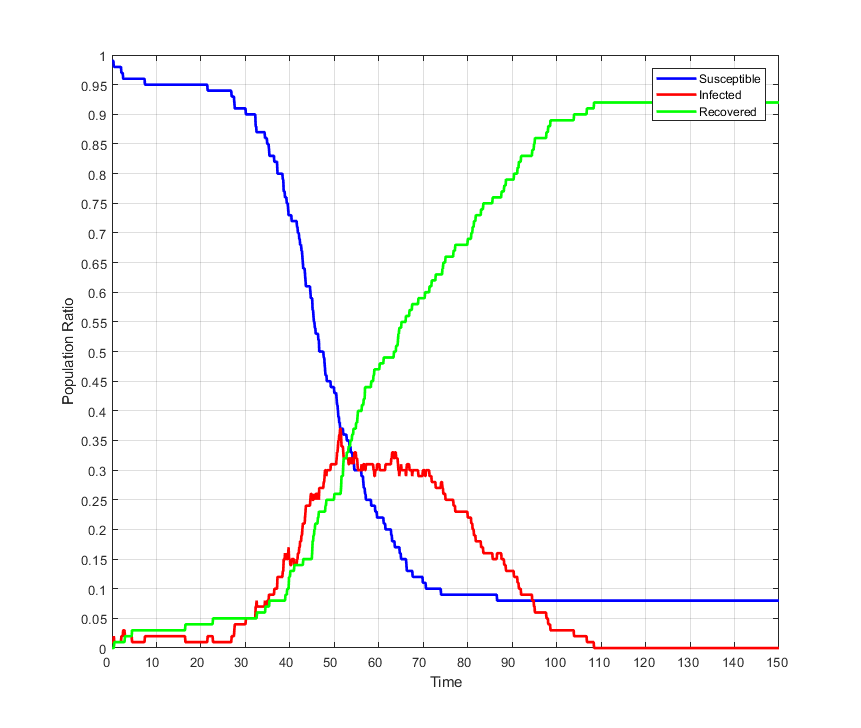
\includegraphics[width=1\textwidth, angle=0]{./fig/step2_yampa/SIR_100agents_150t_01dt.png}
			\caption{100 Agents, $\Delta t = 0.1$}
			\label{fig:sir_abs_approximating_01dt_100agents}
		\end{subfigure}
    	&
		\begin{subfigure}[b]{0.3\textwidth}
			\centering
			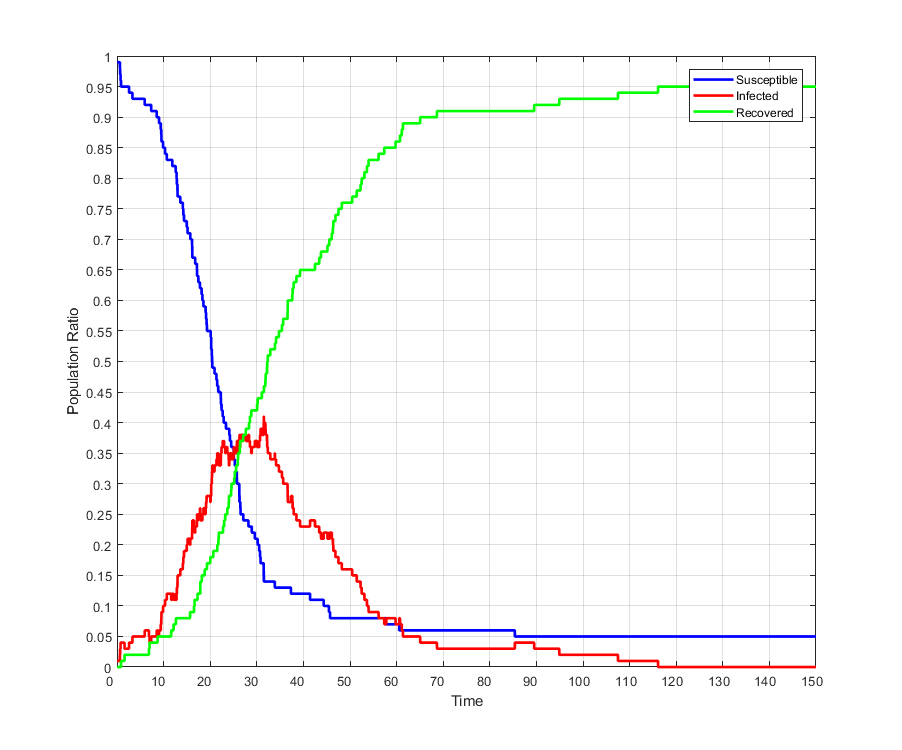
\includegraphics[width=1\textwidth, angle=0]{./fig/step2_yampa/SIR_100agents_150t_001dt.png}
			\caption{100 Agents, $\Delta t = 0.01$}
			\label{fig:sir_abs_approximating_001dt_500agents}
		\end{subfigure}
    	
    	\\
    	
		\begin{subfigure}[b]{0.3\textwidth}
			\centering
			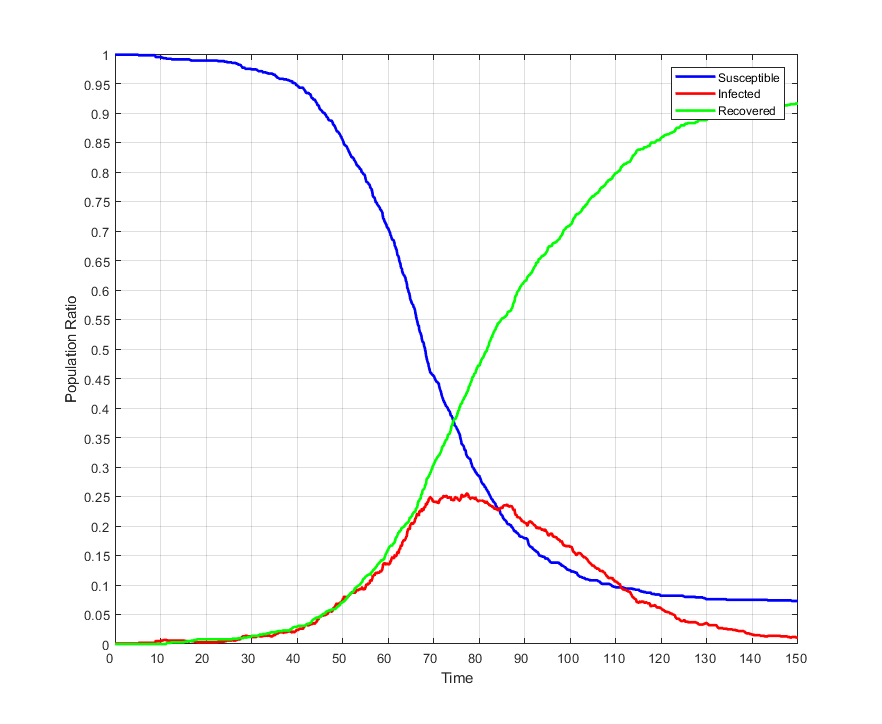
\includegraphics[width=1\textwidth, angle=0]{./fig/step2_yampa/SIR_1000agents_150t_01dt.png}
			\caption{1,000 Agents, $\Delta t = 0.1$}
			\label{fig:sir_abs_approximating_01dt_1000agents}
		\end{subfigure}
		& 
		\begin{subfigure}[b]{0.3\textwidth}
			\centering
			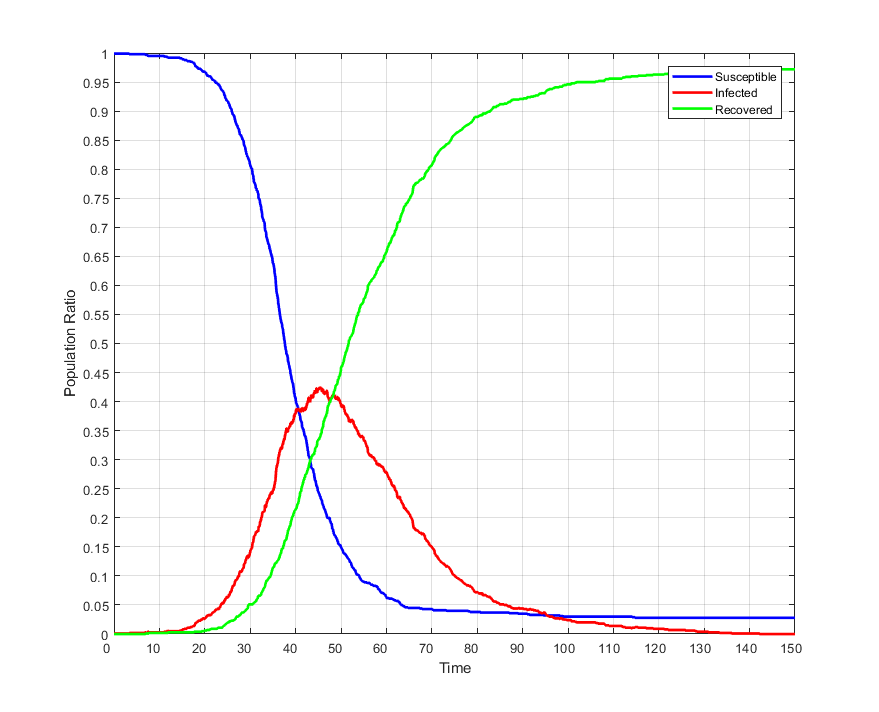
\includegraphics[width=1\textwidth, angle=0]{./fig/step2_yampa/SIR_1000agents_150t_001dt.png}
			\caption{1,000 Agents, $\Delta t = 0.01$}
			\label{fig:sir_abs_approximating_001dt_1000agents}
		\end{subfigure}
	\end{tabular}
	
	\caption{FRP simulation of SIR using agent-based approach. Population size of 100 and 1,000 with contact rate $\beta = \frac{1}{5}$, infection probability $\gamma = 0.05$, illness duration $\delta = 15$ with initially 1 infected agent. Simulation run for 150 time-steps with various $\Delta t$.} 
	\label{fig:sir_abs_dynamics_frp}
\end{center}
\end{figure}

Clearly by keeping the population size constant and just increasing the $\Delta t$ results in a closer approximation to the SD dynamics. Although the dynamics of Figure \ref{fig:sir_abs_approximating_001dt_1000agents} with 1000 agents and $\Delta t = 0.01$ look pretty close to SD, we are still not yet there. We would need to both decrease the sampling rate and increase the number of agents. Unfortunately at this point we are running into severe performance and memory problems because the whole system has to be sampled at an even finer $\Delta t$ whereas we only need to sample occasionally with higher frequency. A possible solution would be to implement super-sampling which would allow us to run the whole simulation with $\Delta t = 1.0$ and only sample the occasionally function with a much higher frequency. An approach would be to introduce a new function to Yampa which allows to super-sample other signal-functions. 

\begin{minted}[fontsize=\footnotesize]{haskell}
superSampling :: Int -> SF a b -> SF a [b]
\end{minted}

It evaluates \textit{sf} for \textit{n} times, each with $\Delta t = \frac{\Delta t}{n}$ and the same input argument \textit{a} for all \textit{n} evaluations. At time 0 no super-sampling is performed and just a single output of \textit{sf} is calculated. A list of \textit{b} is returned with length of \textit{n} containing the result of the \textit{n} evaluations of \textit{sf}. If 0 or less super samples are requested exactly one is calculated. We could then just wrap the occasionally function which would then generate a list of events. We have investigated super-sampling more in-depth but have to leave this due to lack of space.

\subsubsection{Discussion}
By moving on to FRP using Yampa we made a huge improvement in clarity, expressivity and robustness of our implementation. State is now implicitly encoded, depending on which signal-function is active. Also by using explicit time-semantics with \textit{occasionally} we can achieve extremely fine grained stochastics. Compared to drawing a random number of events we create only a single event or none at all. This requires to sample the system with a much smaller $\Delta t$: we are treating it as a truly continuous system, resulting in a hybrid SD/ABS approach.
Still we are not too happy about our approach as we feed back all agents states into every agent, something we want to omit in an agent-based simulation. We now move on to the next section in which we introduce a more general and much more controlled mechanism for feeding back agent-states. 

\subsection{Step III: Adding data-flow}
- getting rid of feeding all agent-states back into every agent, making data-flows explicit between agents, which is necessary because connections between agents are not fixed at compile time


\subsection{Generalising to Monadic Stream Functions}
TODO: write a bit introductory words for this subsection

\subsubsection{Identity Monad}
We start by making the transition to BearRiver by simply replacing Yampas signal-function by BearRivers which is the same but takes an additional type-parameter \textit{m} which indicates the monad. If we replace this type-parameter with the identity monad we should be able to keep the code exactly the same, except from a few type-declarations, because BearRiver re-implements all necessary functions we are using from Yampa \footnote{This was not quite true at the time we wrote this paper, where \textit{occasionally}, \textit{noiseR} and \textit{dpSwitch} were missing. We simply implemented these functions and created a pull request using git.}.
We start by re-defining our general agent signal-function, introducing the monad (stack) our SIR implementation runs in and the agents signal-function:

\begin{minted}[fontsize=\footnotesize]{haskell}
type Agent m o d = SF m (AgentIn d) (AgentOut o d)
type SIRMonad    = Identity
type SIRAgent    = Agent SIRMonad SIRState SIRMsg
\end{minted}

We also have to add the \textit{SIRMonad} to the existing \textit{stepSimulation} type-declarations and we are nearly done. The function \textit{embed} for running the simulation is not provided by BearRiver but by Dunai which has important implications. Dunai does not know and care about time in MSFs, which is exactly what BearRiver builds on top of MSFs. It does so by adding a \textit{ReaderT Double} which carries the $\Delta t$. This means that \textit{embed} returns a computation in the \textit{ReaderT Double} Monad which we need to run explicitly using \textit{runReaderT}. This then results in an identity computation which we simply peel away using \textit{runIdentity}. Here is the complete code of \textit{runSimulation}:

\begin{minted}[fontsize=\footnotesize]{haskell}
runSimulation :: RandomGen g => g -> Time -> DTime -> [(AgentId, SIRState)] -> [[SIRState]]
runSimulation g t dt as = map (map aoObservable) aoss
  where
    steps        = floor (t / dt)
    dts          = replicate steps ()
    n            = length as
    (rngs, _)    = rngSplits g n []
    ais          = map fst as
    sfs          = map (\ (g', (_, s)) -> sirAgent g' ais s) (zip rngs as)
    ains         = map (\ (aid, _) -> agentIn aid) as
    aossReader   = embed (stepSimulation sfs ains) dts
    aossIdentity = runReaderT aossReader dt
    aoss         = runIdentity aossIdentity
\end{minted}

Note that embed does not take a list of $\Delta t$ any more but simply a list of inputs for each step to the top level signal-function.

\subsubsection{Random Monad}
Using the Identity Monad does not gain us anything but it was a first step towards a more general solution. Our next step is to replace the Identity Monad by the Random Monad which will allow us to get rid of the RandomGen arguments to our functions and run the whole simulation within the RandomMonad \textit{again} just as we started but now with the full features functional reactive programming!
We start by re-defining the SIRMonad and SIRAgent:

\begin{minted}[fontsize=\footnotesize]{haskell}
type SIRMonad g = Rand g
type SIRAgent g = Agent (SIRMonad g) SIRState SIRMsg
\end{minted}

Note that we parametrise the Random Monad with a RandomGen g thus this requires to add the RandomGen type-class to all functions where it was not yet added. We also simply remove all RandomGen arguments to all functions except \textit{runSimulation}. The question is now how to access this random monad functionality within the MSF context.
For the function \textit{occasionally}, there exists a monadic pendant \textit{occasionallyM} which requires a MonadRandom type-class. Because we are now running within a MonadRandom instance we simply replace \textit{occasionally} with \textit{occasionallyM}.
Running \textit{gotInfected} is now much easier. Using the function \textit{arrM} of Dunai allows us to run a monadic action in the stack as an arrow. We then directly run gotInfected by lifting it into the random-monad.
This can be seen in the susceptible agent running in the random monad SF:
\begin{minted}[fontsize=\footnotesize]{haskell}
susceptibleAgent :: RandomGen g => [AgentId] -> SIRAgent g
susceptibleAgent ais = switch susceptible(const (infectedAgent))
  where
    susceptible :: RandomGen g => SF (SIRMonad g) SIRAgentIn (SIRAgentOut, Event ())
    susceptible = proc ain -> do
      infected <- arrM (lift . gotInfected infectivity) -< ain
      if infected 
        then returnA -< (agentOut Infected, Event ())
        else (do
          makeContact <- occasionallyM (1 / contactRate) () -< ()
          contactId   <- drawRandomElemSF                   -< ais
          let ao = agentOut Susceptible
          if isEvent makeContact
            then returnA -< (dataFlow (contactId, Contact Susceptible) ao, NoEvent)
            else returnA -< (ao, NoEvent))
\end{minted}

Note also that \textit{drawRandomElemSF} doesn't take a random number generator as well as it has been reimplemented to make full use of the MonadRandom in the stack:

\begin{minted}[fontsize=\footnotesize]{haskell}
drawRandomElemS :: MonadRandom m => SF m [a] a
drawRandomElemS = proc as -> do
  r <- getRandomRS ((0, 1) :: (Double, Double)) -< ()
  let len = length as
  let idx = fromIntegral len * r
  let a =  as !! floor idx
  returnA -< a
\end{minted}

Instead of \textit{noiseR} which requires a RandomGen, it makes use of Dunai \textit{getRandomRS} stream function which simply runs \textit{getRandomR} in the MonadRandom.

Finally because our innermost monad is now the Random Monad instead of the Identity in \textit{runSimulation} we need to replace \textit{runIdentity} by \textit{evalRand}:

\begin{minted}[fontsize=\footnotesize]{haskell}
aossReader = embed (stepSimulation sfs ains) dts
  aossRand = runReaderT aossReader dt
      aoss = evalRand aossRand g
\end{minted}

\subsubsection{Reflections}
By making the transition to MSFs we can now stack arbitrary number of Monads. As an example we could add a StateT monad on the type of AgentOut which would allow to conveniently manipulate the AgentOut e.g. in case where one sends more than one message or the construction of the final AgentOut is spread across multiple functions which allows easy composition. When implementing this one needs to replace the dpSwitch with an individual implementation in which one runs the state monad isolated for each agent.
We could even add the IO monad if our agents require arbitrary IO e.g. reading/writing from files or communicating over TCP/IP. Although one could run in the IO monad, one should not do so as we would loose all guarantees about the reproducibility of our simulation. In ABS we need deterministic behaviour under all circumstances where repeated runs with the same initial conditions, including the random-number generator, should result in the same dynamics. If we allow IO we loose the ability to guarantee the reproducibility at compile-time even if the agents never use IO facilities and just run in the IO for printing debug messages.
So far making the transition to MSFs does not seem as compelling as making the move from the RandomMonad in step 1 to FRP in step 2. Running in the RandomMonad within FRP is convenient but we could achieve the same with passing RandomGen around as we showed in Step 3. In the next step we introduce the concept of a read/write environment which we realise using a StateT monad. This will show the real benefit of the transition to MSFs as without it, implementing a general Environment access would be quite cumbersome.

\subsection{Adding an environment}
In this step we will add an environment in which the agents exist and through which they interact with each other. This is a fundamental different approach to agent-agent interaction but is as valid as the interactions in the previous steps.
In ABS agents are often situated within a discrete 2D environment \cite{schelling_dynamic_1971}, \cite{epstein_growing_1996}, \cite{epstein_agent_zero:_2014} which is simply a finite $N x M$ grid with either a Moore or von Neumann neighbourhood (see Figure \ref{fig:abs_neighbourhoods}). Agents are either static or can move freely around with cells allowing either single or multiple occupants. \\
We can directly map the SIR model to a discrete 2D environment by placing the agents on a corresponding 2D grid with an unrestricted neighbourhood. The behaviour of the agents is the same but they select their neighbours directly from the environment using the provided neighbourhood. Also instead of using data-flow to communicate, agents now communicate through the environment by revealing their current state to their neighbours by placing it on their cell. Agents can read the states of all their neighbours which tells them if a neighbour is infected or not. This allows us to implement the infection mechanism as in the beginning. For purposes of a more interesting and real approach which makes use of the features of agents within an environment, we restrict the neighbourhood to Moore (Figure \ref{fig:moore_neighbourhood}).

\begin{figure}
\begin{center}
	\begin{tabular}{c c}
		\begin{subfigure}[b]{0.3\textwidth}
			\centering
			
\includegraphics[width=0.5\textwidth, angle=0]{./fig/diagrams/neumann.png}
			\caption{von Neumann}
			\label{fig:neumann_neighbourhood}
		\end{subfigure}
    	&
		\begin{subfigure}[b]{0.3\textwidth}
			\centering
			
\includegraphics[width=0.5\textwidth, angle=0]{./fig/diagrams/moore.png}
			\caption{Moore}
			\label{fig:moore_neighbourhood}
		\end{subfigure}
    \end{tabular}
	\caption{Common neighbourhoods in discrete 2D environments of Agent-Based Simulation.}
	\label{fig:abs_neighbourhoods}
\end{center}
\end{figure}

\subsubsection{Implementation}
We start by defining our discrete 2D environment for which we use an indexed two dimensional array. In each cell the agents will store their current state, thus we use the \textit{SIRState} as type for our array data:

\begin{minted}[fontsize=\footnotesize]{haskell}
type Disc2dCoord = (Int, Int)
type SIREnv      = Array Disc2dCoord SIRState
\end{minted}

Next we redefine our monad stack and agent signal-function. We use a StateT transformer on top of our Random Monad from step 4 with the previously defined SIREnv as type for the state. Our agent signal-function now has only unit input and output type as we removed the data-flow mechanism for reasons of clarity. This also indicates through the types that the actions of the agents are only visible in side-effects through the monad stack they are running in.

\begin{minted}[fontsize=\footnotesize]{haskell}
type SIRMonad g = StateT SIREnv (Rand g)
type SIRAgent g = SF (SIRMonad g) () ()
\end{minted}

Instead of having a unique agent id an agent is now initialised through its coordinates in the environment and its initial state. 

\begin{minted}[fontsize=\footnotesize]{haskell}
sirAgent :: RandomGen g => Disc2dCoord -> SIRState -> SIRAgent g
sirAgent c Susceptible = susceptibleAgent c
sirAgent c Infected    = infectedAgent c
sirAgent _ Recovered   = recoveredAgent
\end{minted}

Again the recovered agent behaviour is the shortest one:
\begin{minted}[fontsize=\footnotesize]{haskell}
recoveredAgent :: RandomGen g => SIRAgent g
recoveredAgent = arr (const ())
\end{minted}

The implementation of a susceptible agent is now a bit different and a mix between previous steps. Instead of using data-flows the agent directly queries the environment for its neighbours and randomly selects one of them. The remaining behaviour is similar:

\begin{minted}[fontsize=\footnotesize]{haskell}
susceptibleAgent :: RandomGen g => Disc2dCoord -> SIRAgent g
susceptibleAgent coord = switch susceptible (const (infectedAgent coord))
  where
    susceptible :: RandomGen g => SF (SIRMonad g) () ((), Event ())
    susceptible = proc _ -> do
      makeContact <- occasionallyM (1 / contactRate) () -< ()
      if not (isEvent makeContact)
        then returnA -< ((), NoEvent)
        else (do
          e <- arrM_ (lift get) -< ()
          let ns = neighbours e coord agentGridSize moore
          s <- drawRandomElemS -< ns
          if Infected /= s
            then returnA -< ((), NoEvent)
            else (do
              infected <- arrM_ (lift $ lift $ randomBoolM infectivity) -< ()
              if infected 
                then (do
                  arrM (put . changeCell coord Infected) -< e
                  returnA -< ((), Event ()))
                else returnA -< ((), NoEvent)))
\end{minted}

Note that the susceptible agent itself changes its state in the environment from Susceptible to Infected upon infection.

The behaviour of an infected agent is nearly the same with the difference that upon recovery the infected agent updates its state in the environment from Infected to Recovered.

\begin{minted}[fontsize=\footnotesize]{haskell}
infectedAgent :: RandomGen g => Disc2dCoord -> SIRAgent g
infectedAgent coord = switch infected (const recoveredAgent)
  where
    infected :: RandomGen g => SF (SIRMonad g) () ((), Event ())
    infected = proc _ -> do
      recovered <- occasionallyM illnessDuration () -< ()
      if isEvent recovered
        then (do
          e <- arrM (\_ -> lift get) -< ()
          arrM (\e -> put (changeCell coord Recovered e)) -< e
          returnA -< ((), Event ()))
        else returnA -< ((), NoEvent)
\end{minted}

Running the simulation is now slightly different as we have an initial environment and also need to peel away the StateT transformer:
\begin{minted}[fontsize=\footnotesize]{haskell}
runSimulation :: RandomGen g => g -> Time -> DTime -> SIREnv -> [(Disc2dCoord, SIRState)] -> [SIREnv]
runSimulation g t dt e as = evalRand esRand g
  where
    steps    = floor (t / dt)
    dts      = replicate steps ()
    sfs      = map (uncurry sirAgent) as
    esReader = embed (stepSimulation sfs) dts
    esState  = runReaderT esReader dt
    esRand   = evalStateT esState e
\end{minted}

As initial state we use the initial environment and instead of returning agent states we simply return a list of environments, one for each step. The agent states can then be extracted from each environment.

Due to the different approach of returning the SIREnv in every step, we implemented our own MSF:
\begin{minted}[fontsize=\footnotesize]{haskell}
stepSimulation :: RandomGen g => [SIRAgent g]-> SF (SIRMonad g) () SIREnv
stepSimulation sfs = MSF (\_ -> do
  res <- mapM (`unMSF` ()) sfs
  let sfs' = fmap snd res
  e <- get
  let ct = stepSimulation sfs'
  return (e, ct))
\end{minted}

TODO: if enough space, maybe show implementation of neighbours and changeCell

\subsubsection{Results}
We implemented rendering of the environments using the gloss library which allows us to cycle arbitrarily through the steps and inspect the spreading of the disease over time visually as in Figure \ref{fig:sir_env}.

\begin{figure}
\begin{center}
	\begin{tabular}{c c}
		\begin{subfigure}[b]{0.3\textwidth}
			\centering
			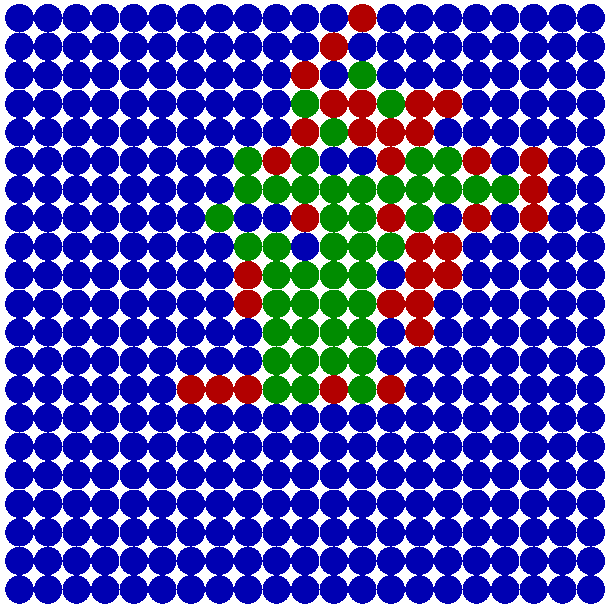
\includegraphics[width=1\textwidth, angle=0]{./fig/step5_environment/SIR_environment_30x30agents_t50_01dt.png}
			\caption{$t = 50$}
			\label{fig:sir_env_t50}
		\end{subfigure}
    	&
		\begin{subfigure}[b]{0.3\textwidth}
			\centering
			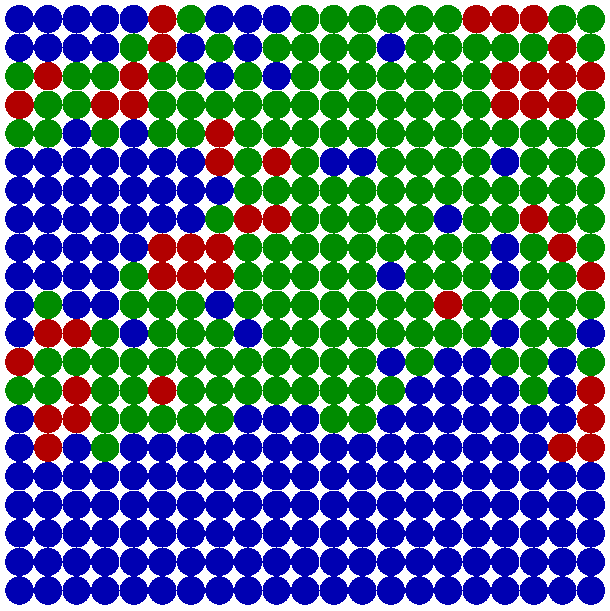
\includegraphics[width=1\textwidth, angle=0]{./fig/step5_environment/SIR_environment_30x30agents_t100_01dt.png}
			\caption{$t = 100$}
			\label{fig:sir_env_t100}
		\end{subfigure}
    	
    	\\
    	
		\begin{subfigure}[b]{0.3\textwidth}
			\centering
			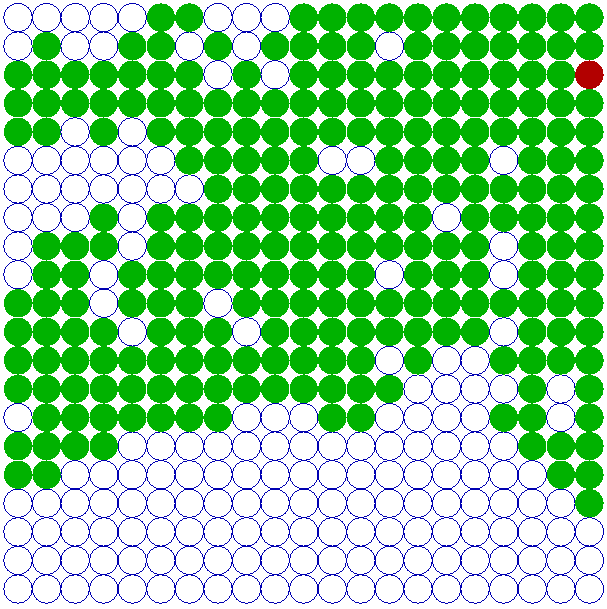
\includegraphics[width=1\textwidth, angle=0]{./fig/step5_environment/SIR_environment_30x30agents_t160_01dt.png}
			\caption{$t = 160$}
			\label{fig:sir_env_t160}
		\end{subfigure}
		& 
		\begin{subfigure}[b]{0.3\textwidth}
			\centering
			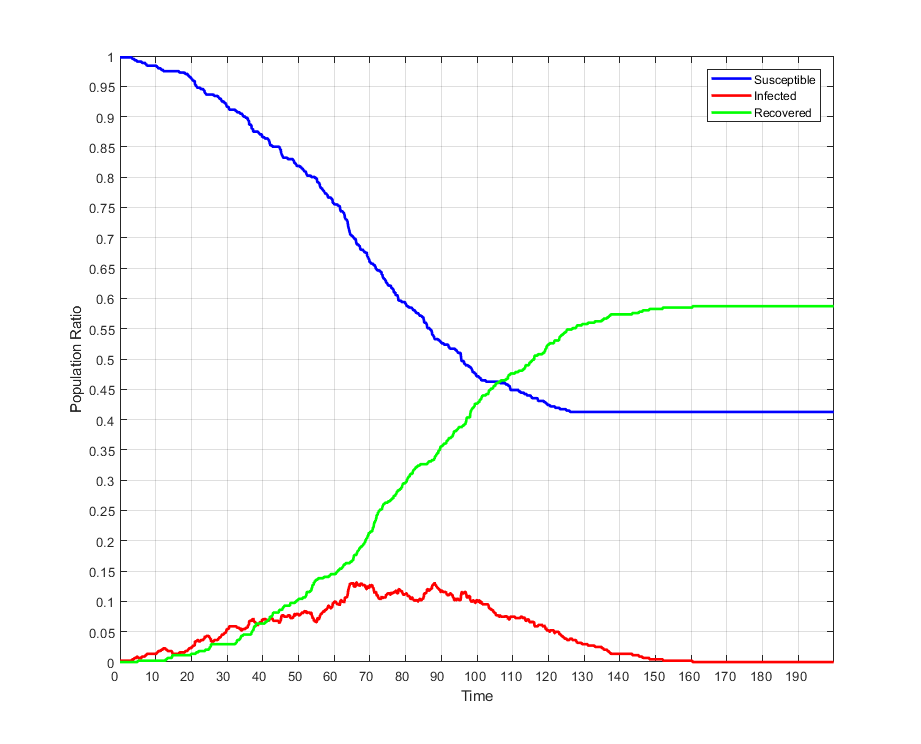
\includegraphics[width=1\textwidth, angle=0]{./fig/step5_environment/SIR_dynamics_30x30agents_300t_01dt.png}
			\caption{Dynamics over time}
			\label{fig:sir_dynamics_30x30agents_300t_01dt}
		\end{subfigure}
	\end{tabular}
	
	\caption{TODO: COLORS!!!! Simulating the agent-based SIR model on a 21x21 2D grid with Moore neighbourhood and a single infected agent at the center and same SIR parameters. Simulation run until $t = 200$ with fixed $\Delta t = 0.1$. Last infected agent recovers around $t = 160$.}
	\label{fig:sir_env}
\end{center}
\end{figure}

Note that the dynamics of the spatial SIR simulation which are seen in Figure \ref{fig:sir_dynamics_30x30agents_300t_01dt} look quite different from the SD dynamics of Figure \ref{fig:sir_sd_dynamics}. This is due to a much more restricted neighbourhood which results in far fewer infected agents at a time and a lower number of recovered agents at the end of the epidemic, meaning that fewer agents got infected overall.

\subsubsection{Discussion}
At first the environment approach might seem a bit overcomplicated and one might ask what we have gained by using an unrestricted neighbourhood where all agents can contact all others. The real win is that we can introduce arbitrary restrictions on the neighbourhood as shown using the Moore neighbourhood. Of course the environment is not restricted to a discrete 2D grid and can be anything from a continuous N-dimensional space to a complex network - one only needs to change the type of the StateT monad and provide corresponding neighbourhood querying functions. The ability to place the heterogeneous agents in a generic environment is also the fundamental advantage of an agent-based over the SD approach and allows to simulate much more realistic scenarios. Note that for reasons of clarity we have removed the data-flow approach from this implementation which results in the unit-types of input and output. In a full blown agent-based simulation library we would combine both approaches.

Generally, there exist four different environment scenarios in an agent-based model
\begin{enumerate}
	\item Passive read-only - implemented in the previous steps, where the environment does never change and is passed as static information, e.g. list of neighbours, to each agent.
	\item Passive read/write - implemented in this step. The environment itself is not modelled as an active process but just as shared data which can be accessed and manipulated by the agents.
	\item Active  read-only - can be implemented by adding an environment agent which broadcasts changes in the environment to all agents using the data-flow mechanism.
	\item Active read/write - can be implemented as in this step plus adding an environment agent which reads/writes the environment e.g. regrowing some resources.
\end{enumerate}

Attempting to introduce an active/passive read/write environment to the Yampa implementation would be quite cumbersome. A possible solution could be to add a type-parameter \textit{e} which captures the type of the environment and then pass it in through the input and allow it to be returned in the output of an agent signal-function. We would then end up with $n$ copies of the environment - one for each agent - which we need to fold back into a single environment. Having an active environment complicates things even further. All these problems are not an issue when using MSFs with a StateT which is a compelling example for making the transition to the more general MSFs. The convenient thing is that although conceptually all agents act at the same time, technically by using \textit{mapM} in stepSimulation they are run after another which also serialises the environment access which gives every agent exclusive read/write access while it is active.

%In the last step we will introduce synchronised agent-transaction as the final agent-agent interaction mechanism. This is a quite sophisticated concept: synchronised agent-transactions which allow an arbitrary number of interactions between two agents without time lag. The use-case for this are price negotiations between multiple agents where the agents need to come to an agreement in the same time-step as described in TODO cite sugarscape.

\subsection{Further Steps}
\subsubsection{Agent-Transactions}
We have implemented synchronous interactions, which we termed agent-transactions in an additional step which we had to omit due to lack of space. Agent-transactions are necessary when an arbitrary number of interactions between two agents need to happen instantaneously without time-lag. The use-case for this are price negotiations between multiple agents where each pair of agents needs to come to an agreement in the same time-step \cite{epstein_growing_1996}. In object-oriented programming, the concept of synchronous communication between agents is implemented directly with method calls. We solved it pure functionally by running the signal functions of the transacting agent pair as often as their protocol requires but with $\Delta t=0$, which indicates the instantaneous character of agent-transactions.

\subsubsection{Dynamic Agent creation}
In the SIR model, the agent population stays constant - agents don't die and no agents are created during simulation - but some simulations \cite{epstein_growing_1996} require dynamic agent destruction and creation. We can easily add and remove agents signal functions in the recursive switch after each time-step. The only problem is that creating new agents requires unique agent ids but with the transition to MSFs we can add a monadic context which allows agents to draw the next unique agent id when they create a new agent. %The id generation process should happen in the agent as the creating agent almost always needs then to communicate with this new agent. If we defer the id generation to the simulation system itself then we need a mechanism to feed it back to the creating agent, which could become quite cumbersome.

% this is omited for now as it takes too much time and involves too many details but would need much more explanation still
%\subsection{Step VI: Adding agent transactions}
Imagine two agents A and B want to engage in a bartering process where agent A, is the seller who wants to sell an asset to agent B who is the buyer. Agent A sends Agent B a sell offer depending on how much agent A values this asset. Agent B receives this sell offer, checks if the price satisfies its utility, if it has enough wealth to buy the asset and replies with either a refusal or its own price offer. Agent A then considers agent Bs offer and if it is happy it replies to agent B with an acceptance of the offer, removes the asset from its inventory and increases its wealth. Agent B receives this acceptance offer, puts the asset in its inventory and decreases its wealth (note that this process could involve a potentially arbitrary number of steps without loss of generality).
We can see this behaviour as a kind of multi-step transactional behaviour because agents have to respect their budget constraints which means that they cannot spend more wealth or assets than they have. This implies that they have to 'lock' the asset and the amount of cash they are bartering about during the bartering process. If both come to an agreement they will swap the asset and the cash and if they refuse their offers they have to 'unlock' them.
In classic OO implementations it is quite easy to implement this as normally only one agent is active at a time due to sequential (discrete event scheduling approach) scheduling of the simulation. This allows then agent A which is active, to directly interact with agent B through method calls. The sequential updating ensures that no other agent will touch the asset or cash and the direct method calls ensure a synchronous updating of the mutable state of both objects with no time passing between these updates.
TODO: this is a novel concept as it is implicitly there already in OO implementations due to global mutual state.

TX: running agents and with 0 dt is easy with bearriver.